\documentclass[12pt]{standalone}

\RequirePackage{times}
\RequirePackage{amsmath}
\RequirePackage{amssymb}
\RequirePackage[T1]{fontenc}

\usepackage{tikz}
\usepackage{xcolor}
\usepackage{pgfplots}
\pgfplotsset{compat=1.16}
\usetikzlibrary{backgrounds,calc,positioning}

\definecolor{red}{HTML}{972e21}
\definecolor{yellow}{HTML}{ebb83f}
\definecolor{blue}{HTML}{7999db}

\begin{document}
	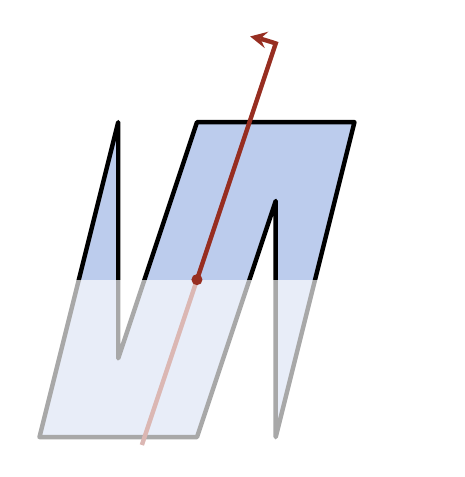
\begin{tikzpicture}[x=1cm,y=1cm]
		\path (-2.15,-2.15) rectangle (3.05,3.2);
		\draw[line join=round,fill=blue!50,ultra thick] (-2,-2) -- (0,-2) -- (1,1) -- (1,-2) -- (2,2) -- (0,2) -- (-1,-1) -- (-1,2) -- cycle;
		\draw[red,ultra thick] (0,0) -- (-0.7,-2.1);
		
		\fill[white,opacity=0.66] let
			\p1=(current bounding box.south west),
			\p2=(current bounding box.south east)
		in
		(\x1,0) -- (\x1,\y1) -- (\x2,\y2) -- (\x2,0) -- cycle;
		
		\fill[red] (0,0) circle (2pt);
		\draw[red,-stealth,ultra thick] (0,0) -- (1,3) arc (71.56505:78:3cm);
	\end{tikzpicture}
\end{document}